%\documentclass[en,hazy,blue,screen,14pt]{elegantnote}
\documentclass[en,hazy,blue]{elegantnote}
\usepackage[T1]{fontenc}
\usepackage[latin9]{inputenc}
% \usepackage[USenglish]{babel}
\usepackage{babel}
\usepackage{float}
\usepackage{textcomp}
\usepackage{amsmath,amsfonts,amssymb}
\usepackage{amsthm}
\usepackage{graphicx}
\usepackage[ruled,vlined]{algorithm2e}
\PassOptionsToPackage{normalem}{ulem}
\usepackage{ulem}
\usepackage{mathtools}
\usepackage{url}
\usepackage{hyperref}
\usepackage{listings}

%%%%%%%%%%%%%%%%%%%%%%%%%%%%%%%%%%%%%%%
% Math Symbols
%%%%%%%%%%%%%%%%%%%%%%%%%%%%%%%%%%%%%%%
\renewcommand{\>}{{\rightarrow}}
\renewcommand{\hat}{\widehat}
\renewcommand{\tilde}{\widetilde}
\newcommand{\half}{\frac{1}{2}}
%
\newcommand{\R}{{\mathbb R}}
\newcommand{\Z}{{\mathbb Z}}
\newcommand{\N}{{\mathbb N}}
\renewcommand{\P}{{\mathbf P}}
\newcommand{\E}{{\mathbf E}}
\newcommand{\Var}{{\mathbf{Var}}}
\newcommand{\I}{{\mathbf I}}
\newcommand{\1}{{\mathbf 1}}
\newcommand{\0}{{\mathbf 0}}
%%%%%%%%%%%%%%%%%%%%%%%%%%%%%%%%%%%%%%%
% Code Style
%%%%%%%%%%%%%%%%%%%%%%%%%%%%%%%%%%%%%%%
\lstset{
	numbers=left, 
	numberstyle=\small, 
	numbersep=8pt, 
	frame = single, 
	framexleftmargin=15pt,
	breaklines=true,
	columns=fullflexible
}
%%%%%%%%%%%%%%%%%%%%%%%%%%%%%%%%%%%%%%%
% Theorem
%%%%%%%%%%%%%%%%%%%%%%%%%%%%%%%%%%%%%%%
\renewcommand\qedsymbol{$\blacksquare$}
\DeclarePairedDelimiter{\ceil}{\lceil}{\rceil}
\newcommand\tab[1][1cm]{\hspace*{#1}}
\newenvironment{claim}[1]{\par\noindent\underline{Claim:}\space#1}{}
\newenvironment{claimproof}[1]{\par\noindent\underline{Proof:}\space#1}{\hfill $\blacksquare$}

%%%%%%%%%%%%%%%%%%%%%%%%%%%%%%%%%%%%%%%
% Title
%%%%%%%%%%%%%%%%%%%%%%%%%%%%%%%%%%%%%%%
\title{Class Notes: STAT 501\\ Nonparametrics \& Log-Linear Models\\ Relative Risk, Odds Ratio, \\Fisher's Exact Test of 2x2 Tables
}
\author{Da Kuang}
\institute{University of Pennsylvania}
% \version{1.00}
\date{}

\begin{document}

\maketitle
\newpage
\tableofcontents

\newpage   
\section{Relative Risk}
A difference between two proportions of a certain fixed size usually is
more important when both proportions are near 0 or 1 than when
they are near the middle of the range.

Consider a comparison of two drugs on the proportion of
subjects who had adverse reactions when using the drug.
\begin{itemize}
	\item The difference between 0.010 and 0.001 is the same as the
difference between 0.410 and 0.401, namely 0.009.
	\item The first difference is more striking, since 10 times as many
subjects had adverse reactions with one drug as the other.
\end{itemize}

In such cases, the ratio of proportions, namely relative risk, is a more relevant descriptive measure. For the above example,

\begin{itemize}
	\item The proportions 0.010 and 0.001 have a relative risk of 0.010/0.001 = 10.
	\item The proportions 0.410 and 0.401 have a relative risk of 0.010/0.001 = 1.02.
\end{itemize}

A relative risk of 1.00 occurs when $p_1 = p_2$, that is when the response is independent of the group.

\section{Review: Study Design}
\subsection{Conditional Design}
When the rows of a contingency table refer to different groups,
the sample sizes for those groups are often fixed by the sampling
design. We assume a binomial distribution for the sample in
each row, with number of trials equal to the fixed row total.

When the columns are a response variable $Y$ and the rows are
an explanatory variable $X$, it is sensible to divide the cell counts
by the row totals to form conditional distributions on the
response. In doing so, we inherently treat the row totals as fixed
and analyze the data the same way as if the two rows formed
separate samples.

\subsection{Unconditional Design}
When the total sample size n is fixed and we cross classify the
sample on two categorical response variables, the multinomial
distribution is the actual joint distribution over the cells. The
cells of the contingency table are the possible outcomes, and the
cell probabilities are the multinomial parameters.
\section{Odds Ratio}
In lecture 9, we assume the rows of contingency table are two independent binomial distributions, and we would like to check whether the two distribution have the same probability parameter.

In this lecture, we would like to exam the dependency. For conditional design, we check the dependency between the two binomial distribution for each row. For the unconditional design, we check the dependency among the four cells in the table.One common used measure for association/dependency is the sample odds ratio.

\subsection{Odds}
For a probability of success $\pi_1$, the odds of success are defined to be $\pi_1 / (1 - \pi_1)$. For instance, if $\pi_1 = 0.75$, the odds of success equal 3.

The odds are non-negative, with value greater than 1 when a success is more likely than a failure.
\begin{itemize}
	\item When odd = $3$, a success is 3 times as likely as a failure. We expect to observe 3 successes for every 1 failure.
	\item When odd = $1/3$, a failure is 3 times as likely as a success. We expect to observe 1 success for every 3 failure.
\end{itemize}

\subsection{Odds Ratio}
Suppose
\begin{itemize}
	\item Random variable $U$ has probability of success $\pi_1$.
	\item Random variable $V$ has probability of success $\pi_2$.
\end{itemize}
\begin{definition}[Odds Ratio]
	Odds ratio is the ratio of two odds
	\[\theta = \frac{\frac{\pi_1}{1 - \pi_1}}{\frac{\pi_2}{1 - \pi_2}} \ge 0\]
\end{definition}

If $\pi_1 = \pi_2$, then $\theta = 1$. The independence of $U$ and $V$ $\iff$ $\theta = 1$.

\subsection{Conditional Design}
Suppose the treatment group subjects iid Bernoulli($\pi_1$), $i = 1, \cdots, n_1$, and the control group subjects iid Bernoulli($\pi_2$), $j = 1, \cdots, n_2$.
\begin{figure}[H]
	\centering
	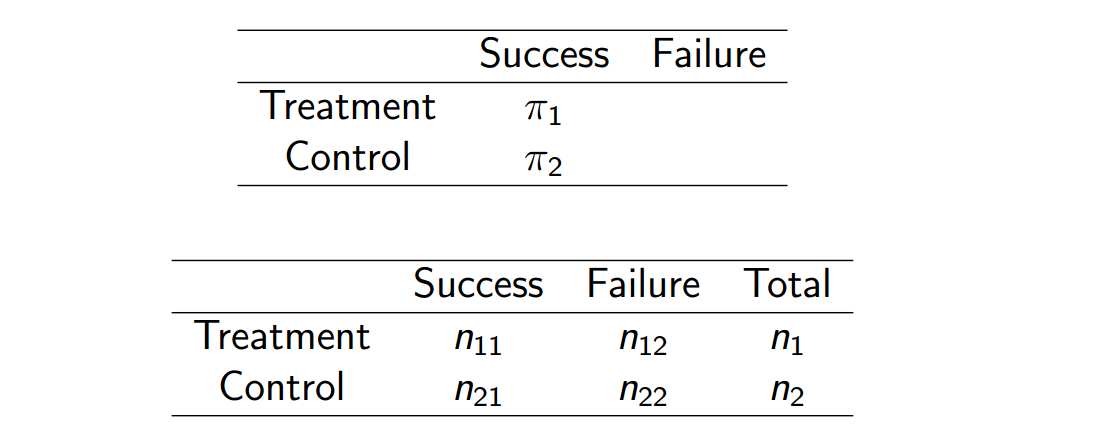
\includegraphics[width=0.7\linewidth]{fig/screenshot001}
	\caption{Conditional Contingency Table}
	\label{fig:screenshot001}
\end{figure}

The sample odd ratio is 
\[\hat{\theta} = \frac{\frac{\pi_1}{1 - \pi_1}}{\frac{\pi_2}{1 - \pi_2}} = \frac{\frac{n_{11}}{n_{12}}}{\frac{n_{21}}{n_{22}}} = \frac{n_{11}n_{22}}{n_{12}n_{21}}\]

\subsection{Unconditional Design}
Let $\pi_{ij}$ denote the true unknown joint probability of falling into the $ij$-th cell, $i=1,2$, $j=1,2$. The contingency table is as follows.

\begin{figure}[H]
	\centering
	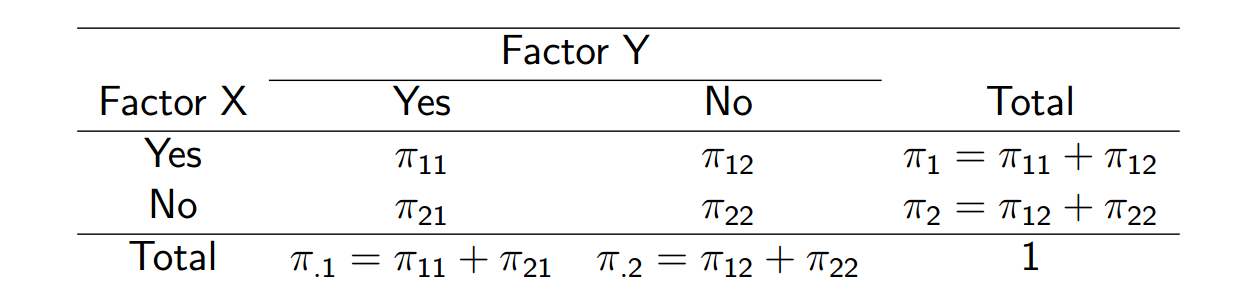
\includegraphics[width=0.7\linewidth]{fig/screenshot002}
	\caption{Unconditional Contingency Table}
	\label{fig:screenshot002}
\end{figure}

In the table, 
\begin{itemize}
	\item $\pi_{11} = \P(X = 1 \text{ and } Y = 1)$
	\item $\pi_{12} = \P(X = 1 \text{ and } Y = 1)$
	\item $\pi_{21} = \P(X = 0 \text{ and } Y = 1)$
	\item $\pi_{22} = \P(X = 0 \text{ and } Y = 0)$
\end{itemize}

The odd $\theta_1$ in the first row is 
\[\theta_1 = \frac{\P(Y = 1 | X = 1)}{P(Y = 0 | X = 1)} = \frac{\frac{\P(Y = 1, X = 1)}{\P(X = 1)}}{\frac{\P(Y = 0, X = 1)}{\P(X = 1)}} = \frac{\frac{\pi_{11}}{\pi_{11} + \pi_{12}}}{\frac{\pi_{12}}{\pi_{11} + \pi_{12}}} = \frac{\pi_{11}}{\pi_{12}}\]

The odd $\theta_2$ in the second row is 
\[\theta_2 = \frac{\P(Y = 1 | X = 0)}{P(Y = 0 | X = 0)} = \frac{\frac{\P(Y = 1, X = 0)}{\P(X = 0)}}{\frac{\P(Y = 0, X = 0)}{\P(X = 0)}} = \frac{\frac{\pi_{21}}{\pi_{21} + \pi_{22}}}{\frac{\pi_{22}}{\pi_{21} + \pi_{22}}} = \frac{\pi_{21}}{\pi_{22}}\]

Therefore, the population odd ratio is
\[\theta = \frac{\theta_1}{\theta_2} = \frac{\frac{\pi_{11}}{\pi_{12}}}{\frac{\pi_{21}}{\pi_{22}}} = \frac{\pi_{11}\pi_{22}}{\pi_{21}\pi_{22}}\]
Hence, the sample odd ratio is
\[\hat{\theta} = \frac{n_{11}n_{22}}{n_{21}n_{22}}\]

One may notice that the sample odd ratios are the same in two different studies.
\section{Properties of Odds Ratio}
\subsection{Directed Association}
The odds ratio $\theta$ measures the strength of association between $X$ and $Y$.
\begin{itemize}
	\item $1 < \theta < \infty$ implies that the odds of $Y = 1$, given that $X = 1$, is larger than the odds that $Y = 1$, given that $X = 0$.
	\item $0 < \theta < 1$ implies that the odds of $Y = 1$, given that $X = 1$, is smaller than the odds that $Y = 1$, given that $X = 0$.
\end{itemize}

Values of $\theta$ farther from 1 in a given direction represent stronger association.

Note that the association is directed.

\begin{itemize}
	\item The odd ratio does not change value when the table orientation reverses so that the rows become the columns and the columns become the rows.
	\item Two values for $\theta$ represent the same strength of association, but
in opposite directions, when one value is the inverse of the other.
\end{itemize}

\subsection{Example: $\theta = 4$ vs. $\theta = 1/4$}
\begin{itemize}
	\item When the order of the rows is reversed or the order of the
	columns is reversed, the new value of $\theta$ is the inverse of the
	original value.
	\item This ordering is usually arbitrary, so whether we get 4 or 0.25 for
	the odds ratio is merely a matter of how we label the rows and
columns.
\end{itemize}

\subsection{Equivalent to independence}
The odd ratio $\theta = 1$ $\iff$ $X$ and $Y$ are independent.
\begin{proof}
	\begin{itemize}
		\item If $X$ and $Y$ are independent, then
		\begin{align*}
			\theta_1 &= \frac{\P(Y = 1| X = 1)}{P(Y = 0| X = 1)} = \frac{\P(Y = 1)}{\P(Y = 0)}\\
			\theta_2 &= \frac{\P(Y = 1| X = 0)}{P(Y = 0| X = 0)} = \frac{\P(Y = 1)}{\P(Y = 0)}\\
			\theta &= \frac{\theta_1}{\theta_2} = 1
		\end{align*}
		\item If $\theta = 1$, then
		\begin{align*}
			\frac{\P(Y = 1, X = 1)}{\P(Y = 0, X = 1)} 
			&= \frac{\P(Y = 1, X = 0)}{\P(Y = 0, X = 0)} \\
			\frac{\P(Y = 1, X = 1)}{\P(X = 1) - \P(Y = 1, X = 1)} 
			&= \frac{\P(Y = 1, X = 0)}{\P(X = 0) - \P(Y = 1, X = 0)} \\
			\frac{\P(Y = 1, X = 1)}{\P(X = 1) - \P(Y = 1, X = 1)} 
			&= \frac{\P(Y = 1, X = 0)}{1 - \P(X = 1) - \P(Y = 1, X = 0)} \\
			\P(X = 1, Y = 1) &= \P(X = 1)\P(Y = 1)
		\end{align*}
	Hence, we have $X$ and $Y$ are independent.
	\end{itemize}
\end{proof}

Therefore the null hypothesis about independence can be reduced to the odd ratio $\theta = 1$.

\subsection{Example: Aspirin vs Cardiovascular Disease}

The Physicians' Health Study was a five-year randomized study
testing whether regular intake of aspirin reduces mortality from
cardiovascular disease. Every other day, the male physicians
participating in the study took either one aspirin tablet or a placebo.
The study was ``blind'' --- the physicians in the study did not know
which type of pill they were taking.

\begin{figure}[H]
	\centering
	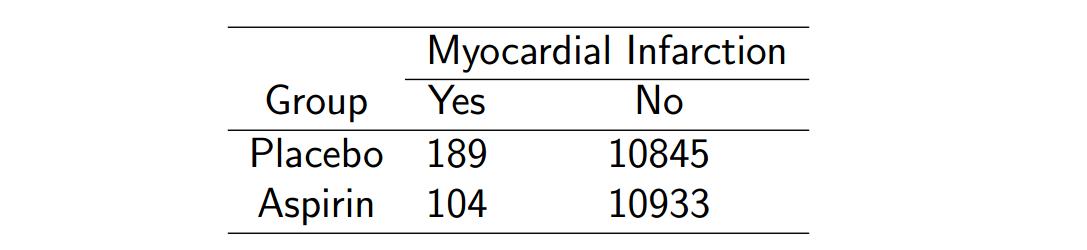
\includegraphics[width=0.7\linewidth]{fig/screenshot003}
	\caption{Preliminary Report: Findings from the Aspirin Component of the Ongoing Physicians' Health Study. New Engl. J. Med., 318: 262-264, 1988.}
	\label{fig:screenshot003}
\end{figure}

\[\theta = \frac{189 \times 10933}{104 \times 10845} = 1.83\]

The estimated odds of Myocardial Infarction for male physicians taking placebo equals
1.83 times the estimated odds for male physicians taking aspirin. The
estimated odds were $83\%$ higher for the placebo group.

\subsection{Large Sample Inference}
If the sample size is large enough, we can use central limit theorem (CLT) for hypothesis testing and estimate the confidence interval.

Note that the range of odd ratio for association is not symmetric, $0 < \theta < 1$ and $1 < \theta < \infty$. So before applying CLT, we need to transform the odd ratio into log-space, i.e. $\lambda = \ln \theta$. 

Then the sample estimation will be $\hat{\lambda} = \ln \hat{\theta}$. The estimated standard deviation is $\hat{\text{SD}} (\hat{\lambda}) = \sqrt{\frac{1}{n_{11}} +\frac{1}{n_{12}} + \frac{1}{n_{21}} + \frac{1}{n_{22}}}$.

The null hypothesis of indepence, $\theta = 1$ can be reduced to $\lambda = 0$.

We can apply CLT to compare $\hat{\lambda}/\hat{\text{SD}} (\hat{\lambda})$ with normal quantile for hypothesis.

Two-sided confidence interval:
\[
	\hat{\lambda} - z_{\alpha/2} \hat{\text{SD}}(\hat{\lambda}) 
	\le \lambda \le
	\hat{\lambda} + z_{\alpha/2} \hat{\text{SD}}(\hat{\lambda}) 
\]

Transform to the odd ratio:
\[
	\exp{(\hat{\lambda} - z_{\alpha/2} \hat{\text{SD}}(\hat{\lambda}))} 
	\le \theta \le
	\exp{(\hat{\lambda} + z_{\alpha/2} \hat{\text{SD}}(\hat{\lambda}))} 
\]

\section{Fisher Exact Test}
Sir Ronald A. Fisher, the English statistician, has been called the
father of modern statistics.

\subsection{The Lady Tasting Tea}
A famous story, in Cambridge, England, in the late 1920is, that a colleague of Fisher's claimed that she
could tell, while drinking tea with milk, whether milk or tea was
poured into the cup first. 

An experiment was designed to test her claim.
\begin{itemize}
	\item 8 cups of tea were presented to her in a random order; 4 of these
	had milk poured first while the other 4 had tea poured first.
	\item She was told that there were 4 cups of each type.
\end{itemize}

Suppose we have the following data show the results of the experiment. 
\begin{figure}[H]
	\centering
	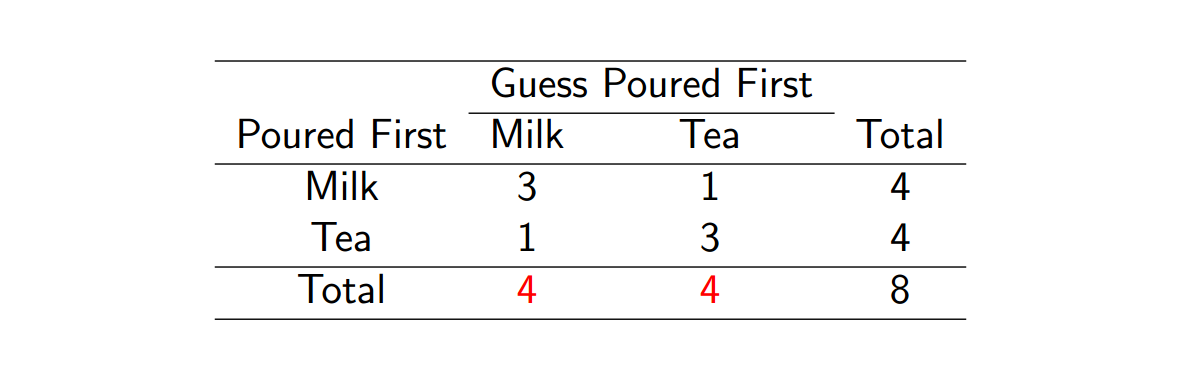
\includegraphics[width=0.7\linewidth]{fig/screenshot004}
	\caption{Contingenvy Table of Lady Tasting Tea}
	\label{fig:screenshot004}
\end{figure}

One can observe that she was right 3 out of 4 times on both types. Is this sufficient
evidence to support her claim of special power?

The contingency table has two difference comparing with the one we met.
\begin{itemize}
	\item The columns are fixed.
	\item The sample size is very small.
\end{itemize}

\subsection{Review: Hyper-geometric Distribution}
Suppose there are $m$ red balls and $n - m$ green balls. We randomly
pick $k$ balls without replacement. What is the probability that $z$ balls
are red?

Let $Z$ be the number of red balls.
\[\P(Z = z) = \frac{{m \choose z} {n-m \choose k - z}}{{n \choose k}}, z = 0, 1, \cdots, k.\]

Here we assume that
\begin{itemize}
	\item $z \le k$
	\item $z \le m$
	\item $k - z \le n - m$
\end{itemize}

\subsubsection{Example}

Suppose we have the following contingency table, in other words, $m = 6$, $n - m = 19$, $n = 25$. Also, $k = 10$ and $z = 1$. 
\begin{figure}[H]
	\centering
	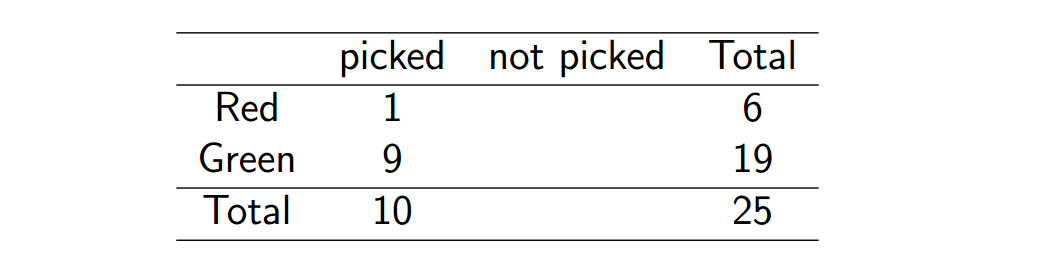
\includegraphics[width=0.7\linewidth]{fig/screenshot005}
	\caption{Hyper-geometric Distribution Example}
	\label{fig:screenshot005}
\end{figure}

We have
\[\P(Z = 1) = \frac{{6 \choose 1}{19 \choose 9}}{{25 \choose 10}}\]

The pdf of hyper-geometric distribution in R is as follows.
\begin{lstlisting}[language=R]
choose(6,1)*choose(19,9)/choose(25,10)
dhyper(x=1, m=6, 19, k=10)
\end{lstlisting}
\subsection{Fisher Exact Test}
Applying the hyper-geometric distribution, conditional on 4 guesses of having milk added first, the probability of
3 correct guesses is
\[\P(Z = 3) = \frac{{4 \choose 3}{4 \choose 4 - 3}}{{8 \choose 4}} = 0.229\]

So if the lady cannot tell the difference between two types of mix, there is still $22.9\%$ of probability for her to have 3 correct guesses by chance. Then how to exam her claim? Hypothesis Testing. To be more specific, Fisher Exact Test.

\subsection{Exact Inference for Small Samples}
The setup of Fisher Exact Test can be represented by the following contingency table.

\begin{figure}[H]
	\centering
	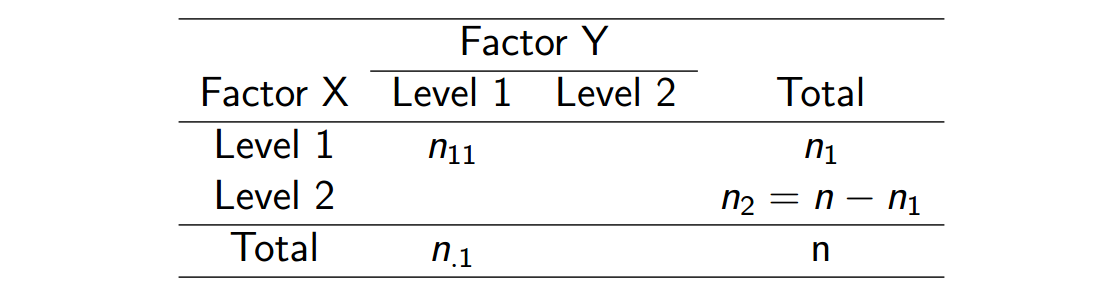
\includegraphics[width=0.7\linewidth]{fig/screenshot006}
	\caption{Contingency Table of Fisher Exact Test}
	\label{fig:screenshot006}
\end{figure}

In the table, $n_1$, $n$, and $n_{.1}$ are fixed. We can infer that $n_{.2} = n - n_{.1}$. $n_{11}$ is the observed random variable.

Fisher's exact test is based on the conditional distribution of $n_{11}$ given $n_1$, $n$, and $n_{.1}$. Given, $z \le \min\{n_1, n_{.1}\}$, and $n_{.1} - z \le n_2$,
\[\P(n_{11} = z) = \frac{{n_1 \choose z} {n_2 \choose n_{.1} - z}}{{n \choose n_{.1}}}.\]

Recall that the $p$-value is calculated by the sum of all event which are equal or rarer than the observed event.

Note that the estimated odd ratio is different from the calculation we have been using. It is because that the experiment design is different with the ones we have. The estimation of odd ratio can be found in R's fisher test manual.
\lstinputlisting[language=R]{code/l10-fisher-exact.R}

\end{document}
